%!TEX TS-program = xelatex

% Шаблон документа LaTeX создан в 2018 году
% Алексеем Подчезерцевым
% В качестве исходных использованы шаблоны
%     Данилом Фёдоровых (danil@fedorovykh.ru)
%        https://www.writelatex.com/coursera/latex/5.2.2
%    LaTeX-шаблон для русской кандидатской диссертации и её автореферата.
%        https://github.com/AndreyAkinshin/Russian-Phd-LaTeX-Dissertation-Template

\documentclass[a4paper,14pt]{article}


%%% Работа с русским языком
\usepackage[english,russian]{babel}   %% загружает пакет многоязыковой вёрстки
\usepackage{fontspec}      %% подготавливает загрузку шрифтов Open Type, True Type и др.
\defaultfontfeatures{Ligatures={TeX},Renderer=Basic}  %% свойства шрифтов по умолчанию
\setmainfont[Ligatures={TeX,Historic}]{Times New Roman} %% задаёт основной шрифт документа
\setsansfont{Comic Sans MS}                    %% задаёт шрифт без засечек
\setmonofont{Courier New}
\usepackage{indentfirst}
\frenchspacing

\renewcommand{\epsilon}{\ensuremath{\varepsilon}}
\renewcommand{\phi}{\ensuremath{\varphi}}
\renewcommand{\kappa}{\ensuremath{\varkappa}}
\renewcommand{\le}{\ensuremath{\leqslant}}
\renewcommand{\leq}{\ensuremath{\leqslant}}
\renewcommand{\ge}{\ensuremath{\geqslant}}
\renewcommand{\geq}{\ensuremath{\geqslant}}
\renewcommand{\emptyset}{\varnothing}

%%% Дополнительная работа с математикой
\usepackage{amsmath,amsfonts,amssymb,amsthm,mathtools} % AMS
\usepackage{icomma} % "Умная" запятая: $0,2$ --- число, $0, 2$ --- перечисление

%% Номера формул
%\mathtoolsset{showonlyrefs=true} % Показывать номера только у тех формул, на которые есть \eqref{} в тексте.
%\usepackage{leqno} % Нумерация формул слева	

%% Перенос знаков в формулах (по Львовскому)
\newcommand*{\hm}[1]{#1\nobreak\discretionary{}
	{\hbox{$\mathsurround=0pt #1$}}{}}

%%% Работа с картинками
\usepackage{graphicx}  % Для вставки рисунков
\graphicspath{{images/}}  % папки с картинками
\setlength\fboxsep{3pt} % Отступ рамки \fbox{} от рисунка
\setlength\fboxrule{1pt} % Толщина линий рамки \fbox{}
\usepackage{wrapfig} % Обтекание рисунков текстом

%%% Работа с таблицами
\usepackage{array,tabularx,tabulary,booktabs} % Дополнительная работа с таблицами
\usepackage{longtable}  % Длинные таблицы
\usepackage{multirow} % Слияние строк в таблице
\usepackage{float}% http://ctan.org/pkg/float

%%% Программирование
\usepackage{etoolbox} % логические операторы


%%% Страница
\usepackage{extsizes} % Возможность сделать 14-й шрифт
\usepackage{geometry} % Простой способ задавать поля
\geometry{top=20mm}
\geometry{bottom=20mm}
\geometry{left=20mm}
\geometry{right=10mm}
%
%\usepackage{fancyhdr} % Колонтитулы
% 	\pagestyle{fancy}
%\renewcommand{\headrulewidth}{0pt}  % Толщина линейки, отчеркивающей верхний колонтитул
% 	\lfoot{Нижний левый}
% 	\rfoot{Нижний правый}
% 	\rhead{Верхний правый}
% 	\chead{Верхний в центре}
% 	\lhead{Верхний левый}
%	\cfoot{Нижний в центре} % По умолчанию здесь номер страницы

\usepackage{setspace} % Интерлиньяж
\onehalfspacing % Интерлиньяж 1.5
%\doublespacing % Интерлиньяж 2
%\singlespacing % Интерлиньяж 1

\usepackage{lastpage} % Узнать, сколько всего страниц в документе.

\usepackage{soul} % Модификаторы начертания

\usepackage{hyperref}
\usepackage[usenames,dvipsnames,svgnames,table,rgb]{xcolor}
\hypersetup{				% Гиперссылки
	unicode=true,           % русские буквы в раздела PDF
	pdftitle={Практическая по БД},   % Заголовок
	pdfauthor={Подчезерцев Алексей},      % Автор
	pdfsubject={Создание и заполнение отношений БД фитнес-клуба},      % Тема
	pdfcreator={Подчезерцев Алексей}, % Создатель
	pdfproducer={Подчезерцев Алексей}, % Производитель
	pdfkeywords={БД} {SQL} {MySQL}, % Ключевые слова
	colorlinks=true,       	% false: ссылки в рамках; true: цветные ссылки
	linkcolor=black,          % внутренние ссылки
	citecolor=black,        % на библиографию
	filecolor=magenta,      % на файлы
	urlcolor=black           % на URL
}
\makeatletter 
\def\@biblabel#1{#1. } 
\makeatother
\usepackage{cite} % Работа с библиографией
%\usepackage[superscript]{cite} % Ссылки в верхних индексах
%\usepackage[nocompress]{cite} % 
\usepackage{csquotes} % Еще инструменты для ссылок

\usepackage{multicol} % Несколько колонок

\usepackage{tikz} % Работа с графикой
\usepackage{pgfplots}
\usepackage{pgfplotstable}

% ГОСТ заголовки
\usepackage[font=small]{caption}
%\captionsetup[table]{justification=centering, labelsep = newline} % Таблицы по правобу краю
%\captionsetup[figure]{justification=centering} % Картинки по центру


\newcommand{\tablecaption}[1]{\addtocounter{table}{1}\small \begin{flushright}\tablename \ \thetable\end{flushright}%	
\begin{center}#1\end{center}}

\newcommand{\imref}[1]{Рис.~\ref{#1}}

\usepackage{multirow}
\usepackage{spreadtab}
\newcolumntype{K}[1]{@{}>{\centering\arraybackslash}p{#1cm}@{}}


\usepackage{xparse}
\ExplSyntaxOn
\DeclareExpandableDocumentCommand{\juliandate}{ m m m }
{
	\juliandate_calc:nnnn { #1 } { #2 } { #3 } { \use:n }
}
\NewDocumentCommand{\storejuliandate}{ s m m m m }
{
	\IfBooleanTF{#1}
	{
		\juliandate_calc:nnnn { #3 } { #4 } { #5 } { \cs_set:Npx #2 }
	}
	{
		\juliandate_calc:nnnn { #3 } { #4 } { #5 } { \cs_new:Npx #2 }
	}
}
\cs_new:Npn \juliandate_calc:nnnn #1 #2 #3 #4 % #1 = day, #2 = month, #3 = year, #4 = what to do
{
	#4 
	{
		\int_eval:n
		{
			#1 +
			\int_div_truncate:nn { 153 * (#2 + 12 * \int_div_truncate:nn { 14 - #2 } { 12 } - 3) + 2 } { 5 } +
			365 * (#3 + 4800 - \int_div_truncate:nn { 14 - #2 } { 12 } ) +
			\int_div_truncate:nn { #3 + 4800 - \int_div_truncate:nn { 14 - #2 } { 12 } } { 4 } -
			\int_div_truncate:nn { #3 + 4800 - \int_div_truncate:nn { 14 - #2 } { 12 } } { 100 } + 
			\int_div_truncate:nn { #3 + 4800 - \int_div_truncate:nn { 14 - #2 } { 12 } } { 400 } -
			32045
		}
	}
}

\tl_new:N \l__juliandate_g_tl
\tl_new:N \l__juliandate_dg_tl
\tl_new:N \l__juliandate_c_tl
\tl_new:N \l__juliandate_dc_tl
\tl_new:N \l__juliandate_b_tl
\tl_new:N \l__juliandate_db_tl
\tl_new:N \l__juliandate_a_tl
\tl_new:N \l__juliandate_da_tl
\tl_new:N \l__juliandate_y_tl
\tl_new:N \l__juliandate_m_tl
\tl_new:N \l__juliandate_d_tl
\int_new:N \l_juliandate_day_int
\int_new:N \l_juliandate_month_int
\int_new:N \l_juliandate_year_int

\cs_new:Npn \__juliandate_set:nn #1 #2
{
	\tl_set:cx { l__juliandate_#1_tl } { \int_eval:n { #2 } }
}
\cs_new:Npn \__juliandate_use:n #1
{
	\tl_use:c { l__juliandate_#1_tl }
}
\cs_new_protected:Npn \juliandate_reverse:n #1
{
	\__juliandate_set:nn { g }
	{ \int_div_truncate:nn { #1 + 32044 } { 146097 } }
	\__juliandate_set:nn { dg }
	{ \int_mod:nn { #1 + 32044 } { 146097 } }
	\__juliandate_set:nn { c }
	{ \int_div_truncate:nn { ( \int_div_truncate:nn { \__juliandate_use:n { dg } } { 36524 } + 1) * 3 } { 4 } }
	\__juliandate_set:nn { dc }
	{ \__juliandate_use:n { dg } - \__juliandate_use:n { c } * 36524 }
	\__juliandate_set:nn { b }
	{ \int_div_truncate:nn { \__juliandate_use:n { dc } } { 1461 } }
	\__juliandate_set:nn { db }
	{ \int_mod:nn { \__juliandate_use:n { dc } } { 1461 } }
	\__juliandate_set:nn { a }
	{ \int_div_truncate:nn { ( \int_div_truncate:nn { \__juliandate_use:n { db } } { 365 } + 1) * 3 } { 4 } }
	\__juliandate_set:nn { da }
	{ \__juliandate_use:n { db } - \__juliandate_use:n { a } * 365 }
	\__juliandate_set:nn { y }
	{
		\__juliandate_use:n { g } * 400 + 
		\__juliandate_use:n { c } * 100 + 
		\__juliandate_use:n { b } * 4 + 
		\__juliandate_use:n { a }
	}
	\__juliandate_set:nn { m }
	{ \int_div_truncate:nn { \__juliandate_use:n { da } * 5 + 308 } { 153 } - 2 }
	\__juliandate_set:nn { d }
	{ \__juliandate_use:n { da } - \int_div_truncate:nn { (\__juliandate_use:n { m } + 4) * 153 } { 5 } + 122 }
	\int_set:Nn \l_juliandate_year_int
	{ \__juliandate_use:n { y } - 4800 + \int_div_truncate:nn { \__juliandate_use:n { m } + 2 } { 12 } }
	\int_set:Nn \l_juliandate_month_int
	{ \int_mod:nn { \__juliandate_use:n { m } + 2 } { 12 } + 1 }
	\int_set:Nn \l_juliandate_day_int
	{ \__juliandate_use:n { d } + 1 }
}
\cs_generate_variant:Nn \juliandate_reverse:n { x }

\NewDocumentCommand{\showday}{ m }
{
	\juliandate_reverse:n { #1 }
	\int_to_arabic:n { \l_juliandate_day_int }-
	\int_to_arabic:n { \l_juliandate_month_int }-
	\int_to_arabic:n { \l_juliandate_year_int }
}

\NewDocumentCommand{\tomorrow}{ }
{
	\group_begin:
	\juliandate_reverse:x { \juliandate_calc:nnnn { \day + 1 } { \month } { \year } { \use:n } }
	\day = \l_juliandate_day_int
	\month = \l_juliandate_month_int
	\year = \l_juliandate_year_int
	\today
	\group_end:
}
\NewDocumentCommand{\tomorrowof}{ m m m }
{
	\group_begin:
	\juliandate_reverse:x { \juliandate_calc:nnnn { #1 + 1 } { #2 } { #3 } { \use:n } }
	\day = \l_juliandate_day_int
	\month = \l_juliandate_month_int
	\year = \l_juliandate_year_int
	\today
	\group_end:
}
\ExplSyntaxOff


\usepackage{xcolor,listings}
\usepackage{textcomp}
\begin{document} % конец преамбулы, начало документа
\begin{titlepage}
	\begin{center}
		ФЕДЕРАЛЬНОЕ  ГОСУДАРСТВЕННОЕ АВТОНОМНОЕ \\
		ОБРАЗОВАТЕЛЬНОЕ УЧРЕЖДЕНИЕ ВЫСШЕГО ОБРАЗОВАНИЯ\\
		«НАЦИОНАЛЬНЫЙ ИССЛЕДОВАТЕЛЬСКИЙ УНИВЕРСИТЕТ\\
		«ВЫСШАЯ ШКОЛА ЭКОНОМИКИ»
	\end{center}
	
	\begin{center}
		\textbf{Московский институт электроники и математики}
		
		\textbf{Им. А.Н.Тихонова НИУ ВШЭ}
		
		\textbf{Департамент электронной инженерии}
	\end{center}	
	\vspace{5ex}
	\begin{center}
\textbf{<<ПОЛУЧЕНИЕ, ОБРАБОТКА И ПРЕДСТАВЛЕНИЕ РЕЗУЛЬТАТОВ МНОГОКРАТНЫХ ИЗМЕРЕНИЙ>>}
	\end{center}	
	\vspace{1ex}
	\begin{center}
\textbf{Отчёт по части 2 лабораторного практикума по дисциплине \\
	<<Электротехника, электроника и метрология>>, раздел <<Метрология>>(ЛР 5-7)}
	\end{center}	
	\vspace{5ex}
	
	\begin{multicols}{2}
	\vfill\null
	\columnbreak
	ВЫПОЛНИЛИ:
	
	Подчезерцев Алексей Евгеньевич
	
	Солодянкин Андрей Александрович
	
	группа БИВ172
	\end{multicols}

	\vfill
	\begin{center}
		Москва \the\year
	\end{center}
\end{titlepage}
\tableofcontents
\pagebreak

\section{ЦЕЛИ РАБОТЫ}
Целями данной работы являются:

\begin{itemize}
    \item получение навыков получения, обработки и представления результатов многократных измерений;
    \item формирование базовых навыков работы в среде NI LabVIEW по раз-работке компонентов для автоматизированной обработки результатов однократных измерений.
\end{itemize}

\section{ПРИМЕНЯЕМОЕ ОБОРУДОВАНИЕ И ПРОГРАММНОЕ ОБЕСПЕЧЕНИЕ}

\begin{enumerate}
    \item    Персональный компьютер (ПК).
    \item    Плата сбора данных NI-DAQ M-series PCI-6221/6251.
    \item    Кабель NI SH68-68-EPM Shielded Cable.
    \item    Коннекторный блок NI BNC 2120
    \item    Провод соединительный коаксиальный (BNC-BNC).
    \item    Среда разработки NI LabVIEW 2013 Professional.
\end{enumerate}


\section{СТРУКТУРА ПРИКЛАДНОГО     ПРОГРАММНОГО ОБЕСПЕЧЕНИЯ}
\subsection{Виртуальный прибор сбора и визуализации данных}

Прибор, изображенный на Рис. \ref{img:av_vi} позволяет измерять напряжение на некотором элементе.
В качестве источника используется блок DAQ Assistant (Рис. \ref{img:av_schema}).

С помощью панели управления можно задать задержку между соседними снятиями сигналов, а так же остановить вычисления.
Снятые значения выводятся на диаграмме в виде точек.
Кроме того, выполняется обработка данных и усреднение результатов за последние 4 измерения, что сглаживает распределение величин.

В конечном счёте пользователь получает два графика -- текущее значение, которое отмечено точками, и усредненное в процессе измерения, обозначенное красной линией.

\begin{figure}[H]
    \centering
    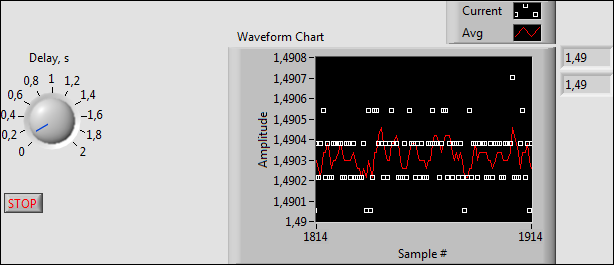
\includegraphics[width=\linewidth]{image/av_vi}
    \caption{Передняя панель Acquire Voltage}\label{img:av_vi}
\end{figure}


\begin{figure}[H]
    \centering
    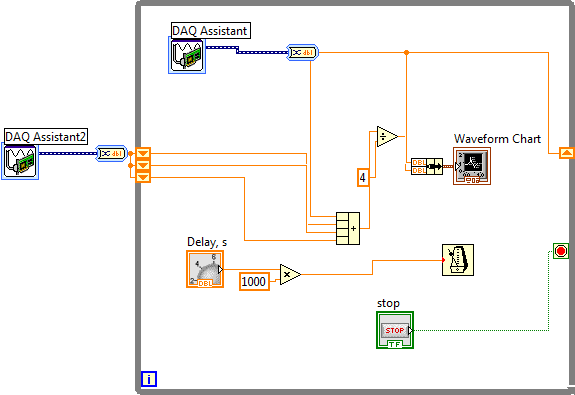
\includegraphics[width=\linewidth]{image/av_schema}
    \caption{Блок-схема Acquire Voltage}\label{img:av_schema}
\end{figure}

\subsection{Виртуальный прибор выполнения многократных измерений }

Передняя панель (Рис. \ref{img:vmm_vi})  по сравнению с предыдущей (Рис. \ref{img:av_vi}) претерпела изменения.
Был отключен вывод усредненного значения на тот же график, добавлен вывод метрик на панель, а именно минимального и максимального значения и среднего.
Кроме того, появилась возможность задавать количество сборов данных через числовое средство ввода <<Number of samples>>.
Добавлен график вывода усредненной информации измерений, при чем усреднение происходит автоматически на каждом участке продолжительностью 0,25 с.
Для удобства дальнейшего редактирования добавлена возможность сохранять полученные данные в файл с помощью элемента выбора файла и индикатора <<Write report>>.
Кроме того, часть измерений выводится напрямую на экран в элемент <<Voltage array>>.

\begin{figure}[H]
    \centering
    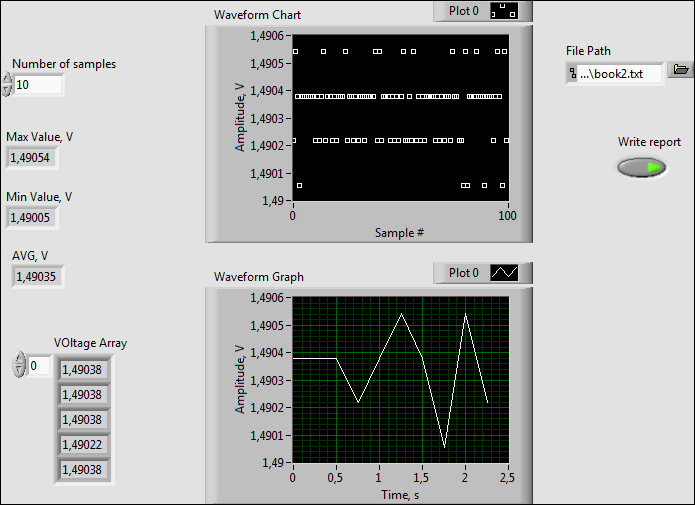
\includegraphics[width=\linewidth]{image/vmm_vi}
    \caption{Передняя панель Voltage Multiple Measurements}\label{img:vmm_vi}
\end{figure}

Под капотом данной VI находится блок схема, представленная на Рис. \ref{img:vmm_schema}.
Количество измерений передается в цикл обработки, далее данные считываются несколько раз с задержкой 250 мс и выводятся на график.
После полученный массив обрабатывается на поиск среднего, минимального и максимального значения, выводится на VI, строимся сгруппированный график с шагом 0,25 с и началом отсчёта в 0 с.
Кроме того, если был выбран пункт сохранения в файл, производится запись с точностью до 5 знаков после запятой.

\begin{figure}[H]
    \centering
    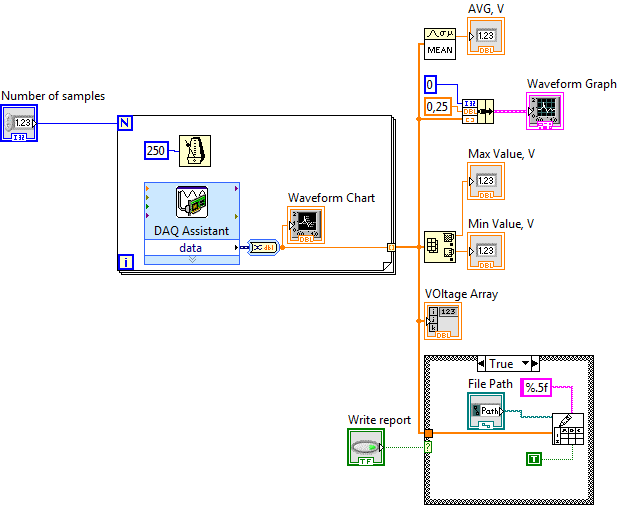
\includegraphics[width=\linewidth]{image/vmm_schema}
    \caption{Блок-схема Voltage Multiple Measurements}\label{img:vmm_schema}
\end{figure}

\subsection{ПРОВЕРКА РЕЗУЛЬТАТОВ ИЗМЕРЕНИЙ НА НАЛИЧИЕ ПРОМАХОВ ПО КРИТЕРИЮ ГРАББСА}

Данная VI (Рис. \ref{img:ot_vi}))предназначена для обработки данных из файла.
С помощью диалогового окна выбирается датасет с результатами некоторых измерений, устанавливается необходимый уровень значимости, который используется при вычислении по критерию Граббса, а так же устанавливается тип сравнения -- критерий Граббса или $3\sigma$.
После выполнения расчетов на верхний график подается изображение исходной выборки, а на нижний -- хороших результатов, прошедших проверку.
Кроме того, в поле <<Array>> попадают значения, отфильтрованные критерием; заполняются поля среднего значения и СКО.

\begin{figure}[H]
    \centering
    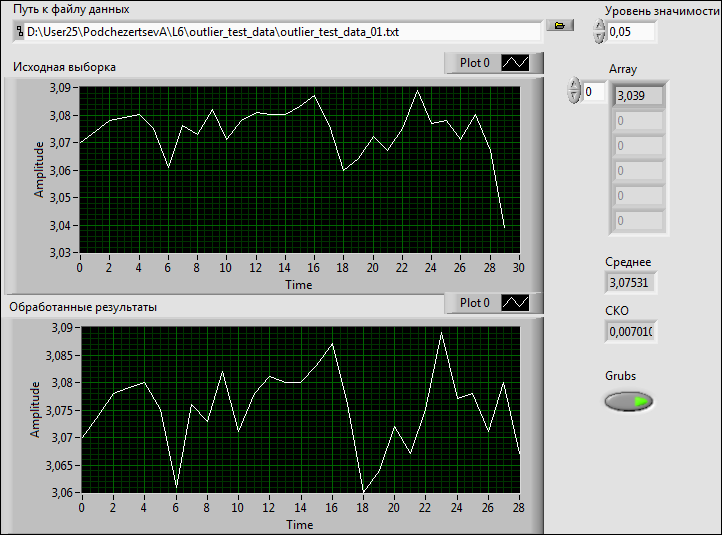
\includegraphics[width=\linewidth]{image/ot_vi}
    \caption{Передняя панель Outlier test}\label{img:ot_vi}
\end{figure}

На рис. \ref{img:ot_schema} представлена блок-схема соответствующей VI.
В данном примере представлен шаг проверки на промахи по критерию $3\sigma$ при отсутствии ошибок.
На рис. \ref{img:ot_schema_init}, \ref{img:ot_schema_err}, \ref{img:ot_schema_stop} представлены шаги инициализации, вычислении ошибок и остановки и являются простыми.
На рис. \ref{img:ot_schema_grubbs} представлен расчет критерия Граббса.
На рис. \ref{img:ot_schema_remove} представлена операция по очистке выборки от промахов.

Обработка данных происходит следующим образом: данные загружаются из файла и выводятся на plot <<Исходная выборка>>.
Далее для данных вычисляется среднее и СКО, затем происходит нормировка и, если все значения удовлетворяют некоторому критерию, выводятся на plot <<Обработанные результаты>>.
Если же есть выбросы, данные обрабатываются еще раз с шага вычисления метрик.
Так происходит до тех пор, пока не будут удовлетворять критерию все данные, после чего вычисления прекращаются.

\begin{figure}[H]
    \centering
    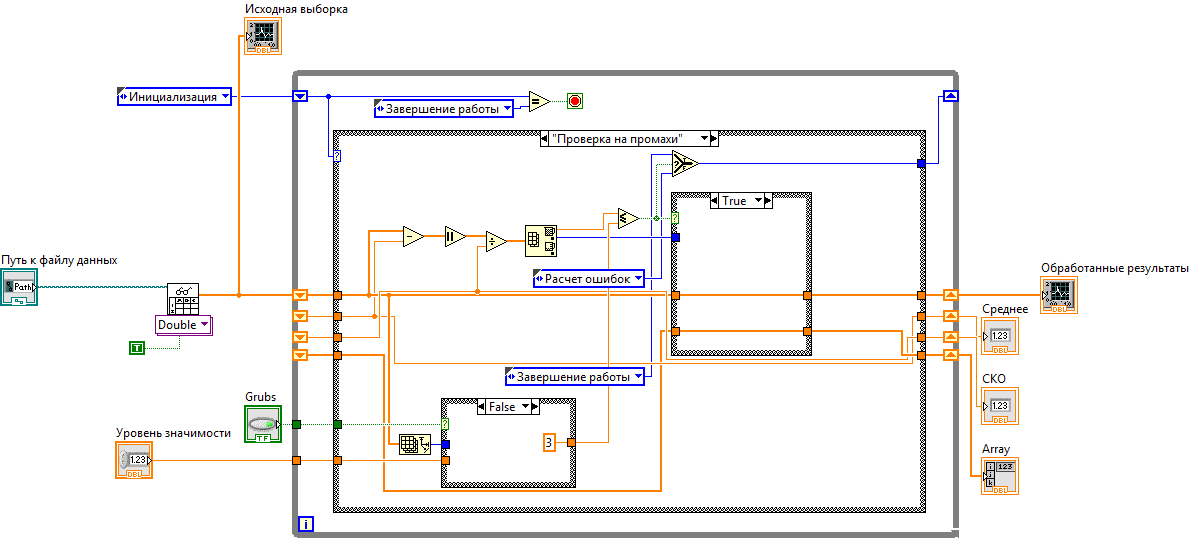
\includegraphics[width=\linewidth]{image/ot_schema}
    \caption{Блок-схема Outlier test}\label{img:ot_schema}
\end{figure}

\begin{figure}[H]
    \centering
    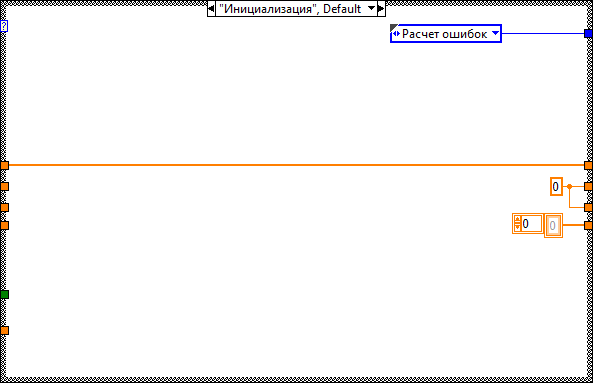
\includegraphics[width=0.5\linewidth]{image/ot_schema_init}
    \caption{Блок-схема Outlier test. Инициализация}\label{img:ot_schema_init}
\end{figure}

\begin{figure}[H]
    \centering
    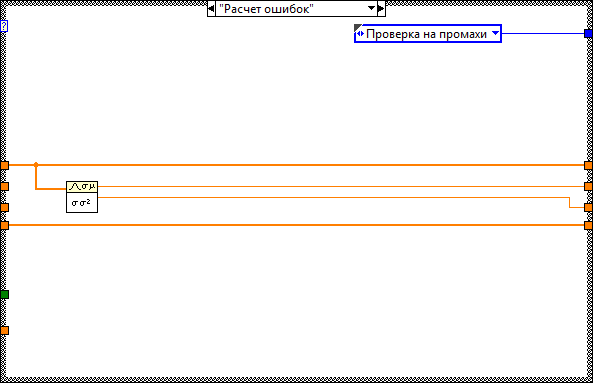
\includegraphics[width=0.5\linewidth]{image/ot_schema_err}
    \caption{Блок-схема Outlier test. Расчет ошибки}\label{img:ot_schema_err}
\end{figure}
\begin{figure}[H]
    \centering
    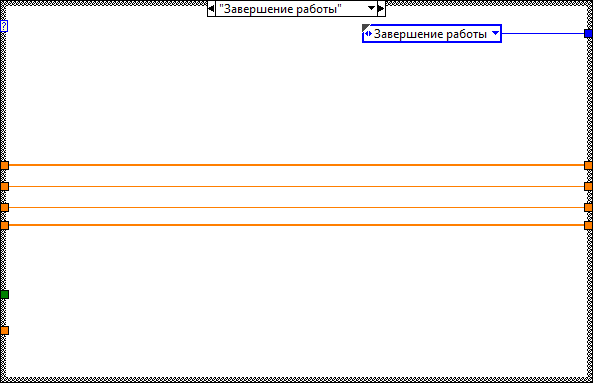
\includegraphics[width=0.5\linewidth]{image/ot_schema_stop}
    \caption{Блок-схема Outlier test. Остановка}\label{img:ot_schema_stop}
\end{figure}
\begin{figure}[H]
    \centering
    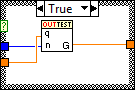
\includegraphics[width=0.3\linewidth]{image/ot_schema_grubbs}
    \caption{Блок-схема Outlier test. Проверка по критерию Граббса}\label{img:ot_schema_grubbs}
\end{figure}

\begin{figure}[H]
    \centering
    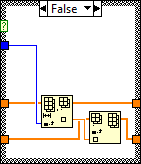
\includegraphics[width=0.3\linewidth]{image/ot_schema_remove}
    \caption{Блок-схема Outlier test. Очистка выборки}\label{img:ot_schema_remove}
\end{figure}

\subsection{ПОЛУЧЕНИЕ, ОБРАБОТКА И ПРЕДСТАВЛЕНИЕ РЕЗУЛЬТАТОВ ПРЯМЫХ МНОГОКРАТНЫХ ИЗМЕРЕНИЙ}

Данная VI (Рис. \ref{img:mp_vi}) позволяет производить анализ множественных измерений.
Исходные данные извлекаются из файла, затем с помощью кнопок управления совершаются соответствующие действия.
Для контроля обработки вручную задаются доверительный интервал и границы неисключенной систематической погрешности.
Итоговый результат записывается в таблицу <<Результат измерений>>, а так же выводится в соответствующее поле с учетом погрешности и строки форматирования.

\begin{figure}[H]
    \centering
    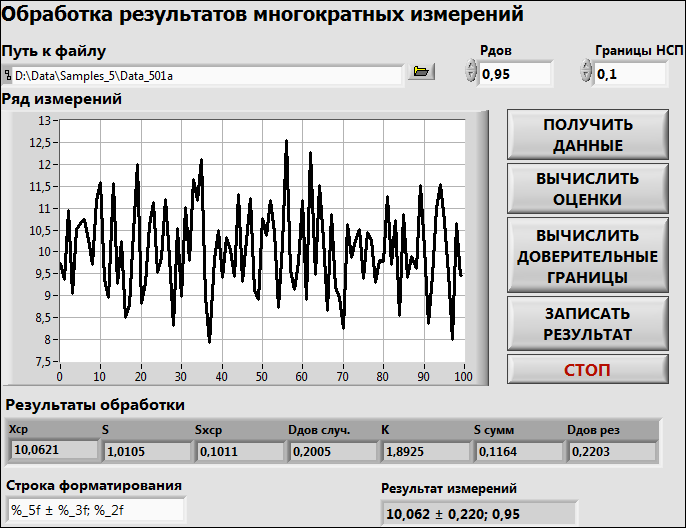
\includegraphics[width=\linewidth]{image/mp_vi}
    \caption{Передняя панель multiple measurements}\label{img:mp_vi}
\end{figure}

На блок-схеме изображен процесс обработки данных (Рис. \ref{img:mp_schema}).
Сначала данные считываются из файла  (Рис. \ref{img:mp_schema_scan}), затем передаются на стадию вычисления оценок.
На этой стадии рассчитываются среднее, СКО,  ошибку  (Рис. \ref{img:mp_schema_calc_score}), записываются в структуру и передаются далее.
После вычисляется доверительный интервал по критерию Стьюдента с учетом уровня значимости и полученных ранее величин (Рис. \ref{img:mp_schema_calc_D}), данные записываются и передаются далее.
На последнем этапе информация форматируется с использованием строки форматирования и выводится на экран результат измерения с учетом погрешности  (Рис. \ref{img:mp_schema_write}).

\begin{figure}[H]
     \centering
     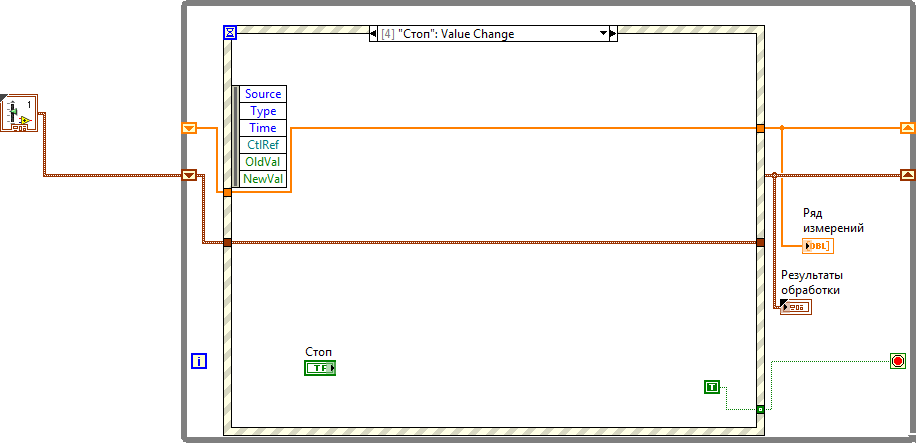
\includegraphics[width=\linewidth]{image/mp_schema}
    \caption{Блок-схема multiple measurements}\label{img:mp_schema}
\end{figure}

  \begin{figure}[H]
     \centering
     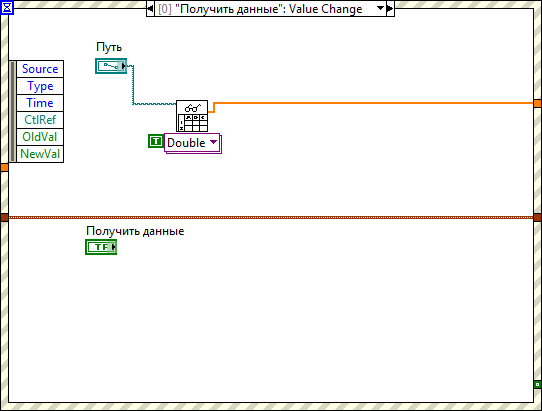
\includegraphics[width=0.7\linewidth]{image/mp_schema_0}
     \caption{Блок-схема multiple measurements. Получение данных}\label{img:mp_schema_scan}
 \end{figure}

 \begin{figure}[H]
    \centering
    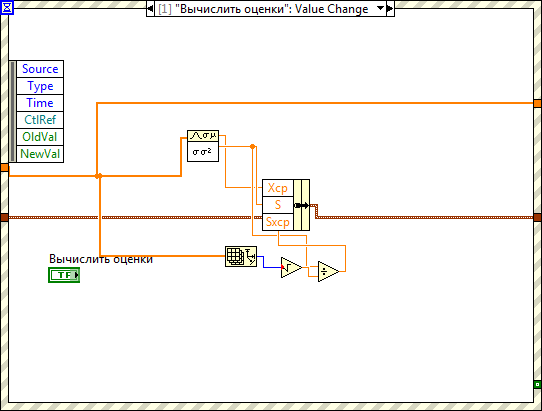
\includegraphics[width=0.7\linewidth]{image/mp_schema_1}
    \caption{Блок-схема multiple measurements. Вычисление оценки}\label{img:mp_schema_calc_score}
\end{figure}
 \begin{figure}[H]
    \centering
    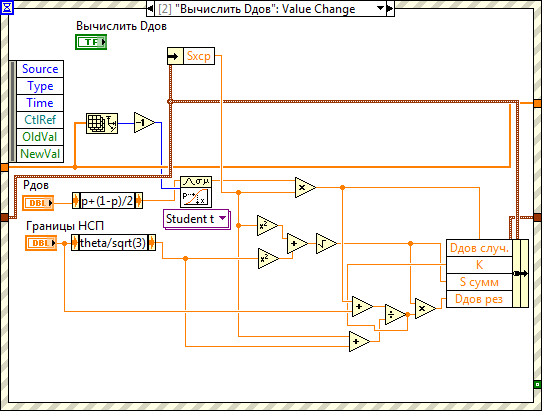
\includegraphics[width=\linewidth]{image/mp_schema_2}
    \caption{Блок-схема multiple measurements. Вычисление доверительного интервала}\label{img:mp_schema_calc_D}
\end{figure}
\begin{figure}[H]
    \centering
    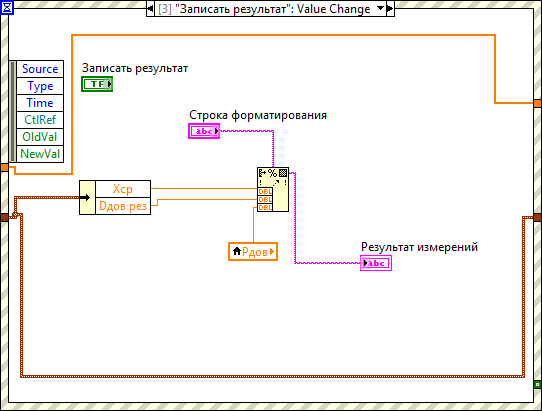
\includegraphics[width=0.7\linewidth]{image/mp_schema_3}
    \caption{Блок-схема multiple measurements. Запись результата}\label{img:mp_schema_write}
\end{figure}
\section{ПОРЯДОК ВЫПОЛНЕНИЯ РАБОТЫ}
\begin{enumerate}
\item     Построение ВП для сбора и визуализации данных на основе Express-VI DAQ Assistant.
 Выполнение сбора и визуализации данных.
 Исследование режимов отображения данных на диаграмме Waveform Chart.
 Экспорт измеренных значений (таблица \ref{tab:av}).
 
\item     Построение ВП для выполнения и сохранения результатов многократных измерений.
 Выполнение многократных измерений, сохранение полученных результатов (таблица \ref{tab:vmm}).
 
\item     Построение ВП для проверки результатов измерений на наличие промахов.
Проверка тестовой выборки (таблица \ref{tab:grubbs_test}), проверка результатов измерений (таблица  \ref{tab:grubbs_train}).

\item     Построение ВП для обработки результатов многократных измерений.
Обработка тестовой выборки (таблица \ref{tab:mm_test}), результатов измерений (таблица \ref{tab:mm_train}).

\end{enumerate}

\section{ РЕЗУЛЬТАТЫ ИЗМЕРЕНИЙ И ВЫЧИСЛЕНИЙ}

\subsection{Результаты сбора данных}

\begin{figure}[H]
	\centering
	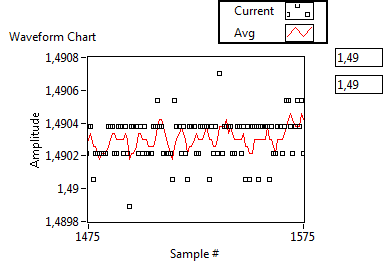
\includegraphics[width=\linewidth]{image/av_graph}
	\caption{График измерений Acquire Voltage}\label{img:av_graph}
\end{figure}

\begin{table}[H]
	\centering
	\caption{Результаты измерений Acquire Voltage}
	\label{tab:av}
	\begin{tabular}{|c|c|}
		\hline
		Номер измерения & Амплитуда, V \\ \hline
		1               & 1,49022      \\ \hline
		2               & 1,49054      \\ \hline
		3               & 1,49054      \\ \hline
		4               & 1,49054      \\ \hline
		5               & 1,49038      \\ \hline
		6               & 1,49038      \\ \hline
		7               & 1,49038      \\ \hline
		8               & 1,49038      \\ \hline
		9               & 1,49022      \\ \hline
		10              & 1,49038      \\ \hline
		11              & 1,49054      \\ \hline
		12              & 1,49022      \\ \hline
		13              & 1,49022      \\ \hline
		14              & 1,49038      \\ \hline
		15              & 1,49022      \\ \hline
		16              & 1,49005      \\ \hline
		17              & 1,49054      \\ \hline
		18              & 1,49022      \\ \hline
		19              & 1,49022      \\ \hline
		20              & 1,49038      \\ \hline
	\end{tabular}
\end{table}

\subsection{Результаты многократных измерений}

Минимум: 1,49005V

Максимум: 1,49054V

Среднее: 1,49035V

\begin{table}[H]
	\centering
	\caption{Результаты измерений Voltage Multiple Measurements}
	\label{tab:vmm}
	\begin{tabular}{|c|c|}
		\hline
		Номер измерения & Амплитуда, V \\ \hline
		1               & 1.49038      \\ \hline
		2               & 1.49038      \\ \hline
		3               & 1.49034      \\ \hline
		4               & 1.49026      \\ \hline
		5               & 1.49026      \\ \hline
		6               & 1.49022      \\ \hline
		7               & 1.49026      \\ \hline
		8               & 1.49026      \\ \hline
		9               & 1.49038      \\ \hline
		10              & 1.49038      \\ \hline
		11              & 1.49038      \\ \hline
		12              & 1.49026      \\ \hline
		13              & 1.49022      \\ \hline
		14              & 1.49022      \\ \hline
		15              & 1.49018      \\ \hline
		16              & 1.4903       \\ \hline
		17              & 1.49038      \\ \hline
		18              & 1.49042      \\ \hline
		19              & 1.49046      \\ \hline
		20              & 1.49046      \\ \hline
	\end{tabular}
\end{table}

\subsection{Результаты проверки на промахи по критерию Граббса}

\begin{table}[H]
	\centering
	\caption{Проверка тестовой выборки}
	\label{tab:grubbs_test}
	\begin{tabular}{|c|c|}
		\hline
		Число измерений                 & 29      \\ \hline
		Среднее арифметическое значение & 3,07531 \\ \hline
		СКО                             & 0,00701 \\ \hline
		Промахи                         & 3,039   \\ \hline
	\end{tabular}
\end{table}

\begin{table}[H]
	\centering
	\caption{Проверка результатов измерений }
	\label{tab:grubbs_train}
	\begin{tabular}{|c|c|}
		\hline
		Число измерений                 & 19       \\ \hline
		Среднее арифметическое значение & 1.49035  \\ \hline
		СКО                             & 0.000144 \\ \hline
		Промахи                         & --       \\ \hline
	\end{tabular}
\end{table}

\subsection{Результаты обработки результатов многократных измерений}

\begin{table}[H]
	\centering
	\caption{Обработка тестовой выборки }
	\label{tab:mm_test}
	\begin{tabular}{|c|c|}
		\hline
		              Наименование параметра                &  Значение параметра  \\ \hline
		                  Число измерений                   &         100          \\ \hline
		        Среднее арифметическое значение, В          &       10.0621        \\ \hline
		               Оценка СКО группы, В                 &        1.0105        \\ \hline
		        Оценка СКО результата измерения, В          &        0.1011        \\ \hline
		             Доверительная вероятность              &         0.95         \\ \hline
		  Доверительные границы случайной погрешности, В    &        0.2005        \\ \hline
		                  Границы НСП, В                    &         0.1          \\ \hline
		                         К                          &        1.8925        \\ \hline
		Доверительные границы оценки измеряемой величины, В &        0.2203        \\ \hline
		              Результат измерений, В                & 10.062 ± 0.220; 0.95 \\ \hline
	\end{tabular}
\end{table}

\begin{table}[H]
	\centering
	\caption{Обработка результатов измерений }
	\label{tab:mm_train}
	\begin{tabular}{|c|c|}
		\hline
		              Наименование параметра                &  Значение параметра   \\ \hline
		                  Число измерений                   &          19           \\ \hline
		        Среднее арифметическое значение, В          &        1.49035        \\ \hline
		               Оценка СКО группы, В                 &        0.0001         \\ \hline
		        Оценка СКО результата измерения, В          & $3.224 \times 10^-5$  \\ \hline
		             Доверительная вероятность              &         0.95          \\ \hline
		  Доверительные границы случайной погрешности, В    & $6.7479 \times 10^-5$ \\ \hline
		                  Границы НСП, В                    &          0.1          \\ \hline
		                         К                          &        1.7323         \\ \hline
		Доверительные границы оценки измеряемой величины, В &          0.1          \\ \hline
		              Результат измерений, В                & 1.4903 ± 0.100; 0.95  \\ \hline
	\end{tabular}
\end{table}
\section{ВЫВОДЫ ПО РАБОТЕ}

В ходе работы были получены следующие результаты:

\begin{itemize}
	\item Были получены данные измерения напряжения в среде LabView, с которыми были подвержены статистической обработке с целью определения погрешности и промахов.
	\item Распределение было проверено по критериям Граббса, $3 \sigma$ и Стьюдента.
	В результате измерений не было найдено выбросов с заданными доверительными интервалами.
	Тем не менее, на специальных тестовых данных выбросы были, что подтверждает работоспособности алгоритма.
	\item Для визуализации данных использовались блоки Waveform Chart и Waveform Graph, которые позволяют выводит зависимости от времени или итерации, размещать несколько графиков на одном plot.
	\item Для статистической обработки использовались как простые функции, возвращающие максимум, минимум, среднее и дисперсию распределения, размер выборки, так и сложные, проверяющие выборку по критерию Граббса или Стьюдента.
	\item Для обработки массивов данных использовались функции статистической обработки, преобразования потока данных от измерительного прибора, добавления или удаления элементов для фильтрации, Bundle or Unbundle by name для извлечение конкретного поля из структуры данных. 
	Кроме того, использовались функции для считывания данных из файла в массив и наоборот.
	\item В данных работах были использованы алгоритмические структуры циклы while, for, оператор множественного выбора switch/case, условный оператор, тернарный оператор (select), константы.
	Для передачи данных от одной итерации цикла к последующим использовались сдвиговые регистры.
	\item Для реализации паттерна конечного автомата использовалась константа со списком всех состояний, цикл while, который останавливался при шаге завершения работы, структура case, в которой были определены действия для каждого случая и следующая итерация в зависимости от ситуации.
\end{itemize}

\end{document} % конец документа